\chapter{Implementierung}
\label{ch:implementierung}

Den Einstieg in das Programm stellt die Datei \Code{main.py} dar.
Hier wird entschieden, ob ein Online- oder Offline-Spiel, wie bereits in den vorherigen Kapiteln beschrieben, gestartet
werden soll.
Die Implementierungen dieser beiden Spielvarianten sollen in diesem Kapitel beschrieben werden, wobei der Fokus auf
die Online-Verbindung gerichtet ist, da es sich hierbei um die Umsetzung der eigentlichen Aufgabenstellung handelt.

\section{Modellierung des Spiels}
\label{sec:modellierung}

Um eine Grundlage zu haben, auf der die Implmentierung aufgebaut werden konnte, wurde zunächst die Modellierung des
Spiels vorgenommen.
Dazu haben wir geschaut, welche Informationen benötigt und vom Server bereitgestellt werden und wie man diese dann
mithilfe eines objektorientierten Ansatzes abbilden kann.

Das Ergebnis der Modellierung ist in \Abbildung{fig:klassendiagramm-modell} zu sehen.
Das \Code{Game} hat Zugriff auf die eigenen Eigenschaften, kennt aber auch alle \Code{Player}, die an diesem Spiel
teilnehmen.
Zudem besteht ein \Code{Game} aus einem zweidimensionalen Array aus \Code{Cells}, die das Spielfeld repräsentieren.
In einer \Code{Cell} können sich dann kein, ein oder nach einer Kollision auch mehrere Spieler befinden.

\begin{figure}[htb]
\centering
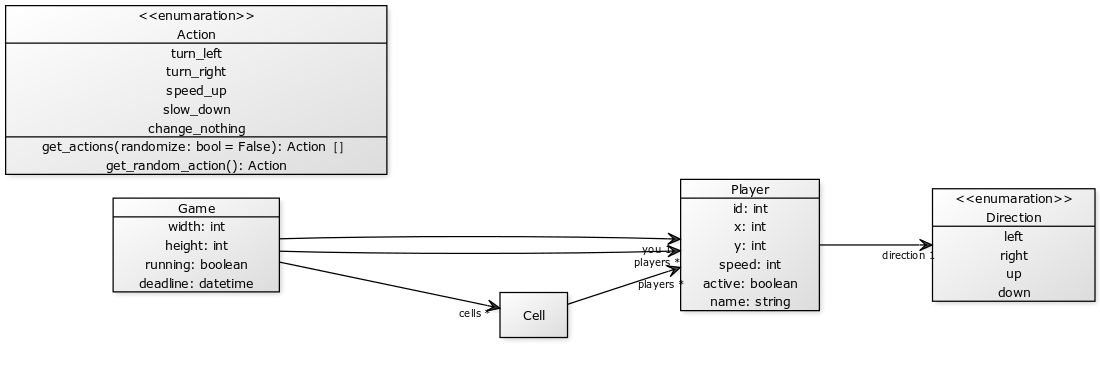
\includegraphics[width=\textwidth]{Bilder/Klassendiagramm_Modellierung.png}
\caption{UML-Klassendiagramm des Modells}
\label{fig:klassendiagramm-modell}
\end{figure}

Da ein Spieler in eine bestimmte Anzahl an Richtungen gedreht sein kann, wird diese Ausrichtung über die Enumeration
\Code{Direction} abgebildet.
Ebenso ist die Auswahl der möglichen Aktionen begrenzt, sodass diese in der Enumeration \Code{Action} festgelegt
worden sind.

\section{Implementierung des Online-Spiels}
\label{sec:online-implementierung}

Um eine Verbindung zu dem \Code{spe\_ed}-Server aufbauen zu können, müssen die URL und ein gültiger API-Key vor dem
Start der Anwendung als Umgebungsvariablen gesetzt worden sein.
Diese Websocket-URL wird entsprechend modifiziert auch als Endpunkt zur Abfrage der Server-Zeit verwendet, auf deren
Nutzung nachfolgend noch eingegangen wird.

Die zum Start des Spiels öffentlich bereitgestellte Methode \Code{play()} ist in \Listing{lst:online-play} dargestellt.
Diese ist sehr simpel und ruft lediglich die private Methode \Code{\_\_play()} auf.
Hierbei handelt es sich um eine asynchrone Methode, wie schon in der Methoden-Signatur deutlich wird.
Es wird mittels der Bibliothek \Code{asyncio} sichergestellt, dass diese asynchrone Methode vollständig verarbeitet
wurde, bevor der Kontrollfluss im Programm weiterläuft.
Sobald dies der Fall ist, ist das Spielende eingetreten und die Oberfläche wird beendet.

\lstinputlisting[label=lst:online-play,language=Python,caption=\Code{play()}-Methode der \Code{OnlineConnection}]
{./Dokumente/OnlineConnection-play.txt}

In der im vorherigen Absatz bereits erwähnten Methode \Code{\_\_play()} in der \Code{OnlineConnection} wird eine
Websocket-Verbindung zum Server aufgebaut.
Anschließend wird in einer Endlosschleife die Logik zur Ausführung eines einzelnen Spielzugs ausgeführt.
Wie ein solcher Spielzug abläuft, ist in \Anhang{fig:sequenzdiagramm-spielzug} in Form eines Sequenzdiagrammes
nachvollziehbar und die Umsetzung in Python-Code kann zusammen mit dem Verbindungaufbau \Listing{lst:online-__play}
entnommen werden.

\lstinputlisting[label=lst:online-__play,language=Python,caption=\Code{\_\_play()}-Methode der \Code{OnlineConnection}]
{./Dokumente/OnlineConnection-__play.txt}

\subsection{Einlesen des Spiel-Zustands}
\label{subsec:einlesen-spielzustand}

Der Beginn einer neuen Spielrunde wird damit eingeläutet, dass neue Daten über die Websocket-Verbindung vom Server
versendet werden.
Dabei handelt es sich jeweils um den aktuellen Zustand des Spiels mit allen notwendigen Daten.
Zur Serialisierung wird das Spiel in ein JSON-Format übersetzt.
Ein Beispiel zur Veranschaulichung dieses Formats ist in \Anhang{lst:json-spiel} abgebildet.
Anzumerken ist, dass die exakte Formatierung des Strings abweichen kann.

Dieser eingelesene String wird an ein Objekt der Klasse \Code{JSONDataLoader} übergeben, welches die Übersetzung des
JSON-Formats in ein \Code{Game}-Objekt - das wie in \Kapitel{sec:modellierung} beschrieben modelliert ist - zur Aufgabe
hat.

Sobald das Spiel fertig aufgebaut wurde, wird ein \Code{GET}-Request an den Server geschickt, auf welchen als Antwort
die aktuelle Server-Zeit erwartet wird und ebenfalls durch den \Code{JSONDataLoader} aus einem String in ein
\Code{datetime}-Objekt geparst wird.
Diese Server-Zeit wird dann verwendet, um durch einen Abgleich mit der Zeit des eigenen Systems gegebenenfalls die
Deadline für die Festlegung auf die nächste Aktion zu verschieben, da diese sich immer nach der Server-Zeit richtet.
Es wird hierbei eine Toleranz von drei Sekunden eingebaut, da je nach Internet-Verbindung die Anfrage an den Server
etwas dauern kann und so die Aktion besser zu früh als zu spät übermittelt werden sollte.

\subsection{Ermittelung der besten Aktion}
\label{subsec:ermitteln-aktion}

Anschließend ist das Spiel in seinem aktuellen Zustand korrekt abgebildet.
Als nächstes steht an, dass eine Entscheidung für die nächste Aktion getroffen werden muss.
Dies ist allerdings nur notwendig, wenn der eigene Spieler noch aktiv ist.

Die Berechnung und Festlegung auf die nächste Aktion wird von der \Code{OnlineConnection} an ein Objekt einer
Subklasse der abstrakten Basisklasse \Code{ArtificialIntelligence} mit dem Aufruf der Methode
\Code{create\_next\_action(game: Game)} deligiert.
Welche Art der im \Kapitel{ch:loesungsansatz} beschriebenen \ac{KI}s gewählt werden soll, steht dem Anwender
grundsätzlich vollkommen frei.

\subsection{Übergabe der Aktion an die Web-API}
\label{subsec:uebergabe-aktion}

Sobald eine Aktion ausgewählt wurde, muss diese dem Server noch mitgeteilt werden.
In der Dokumentation für die diesjährige Aufgabestellung wurde festgehalten, dass auch hier wieder das JSON-Format
verwendet werden soll.
Daher wird die Aktion an die Klasse \Code{JSONDataWriter} überreicht, die einen String folgender Form erstellt:
\texttt{\{\dq action\dq : \dq speed\_up\dq \}}, welcher dann über die Websocket-Verbindung an der Server gesendet wird.

\section{Implementierung des Offline-Spiels}
\label{sec:offline-implementierung}

Bei der Offline-Version des Spiels ging es darum, lokal die eigenen \ac{KI}s gegeneinander und
als menschlicher Spieler gegen die \ac{KI} antreten zu können, ohne eine Verbindung zum spe\_ed-Server herzustellen.
Dies ermöglichte uns lokal zu testen und unsere verschiedenen Lösungsansätzen (siehe \Kapitel{ch:loesungsansatz})
gegeneinander spielen zu lassen, um zu beurteilen, welche die Beste ist.
Die Implementierung des Offline-Spiels erfolgte in der Klasse \Code{OfflineConnection}, die entsprechend der Ober-Klasse
\Code{Connection}, die Methode \Code{play()} implementiert. \\

Da wir keine Verbindung zum spe\_ed-Server herstellen, erhalten wir keine Aktualisierung des Spiels.
Auch müssen die errechneten Aktionen der \ac{KI} nicht versendet, sondern lokal verarbeitet werden.
Daher haben wir die Spiellogik in der Klasse \Code{GameService} nachgebildet.
Diese Klasse manipuliert das übergebene Spiel und ist somit der Ersatz zum spe\_ed-Server in der Offline-Variante.
Die Klasse \Code{GameService} muss folglich in der oben genannten Methode \Code{play()}, der \Code{OfflineConnection},
initialisiert werden.
Dazu müssen zunächst \Code{Player}-Objekte und das entsprechende \Code{Game}-Objekt erzeugt werden, welches dem
\Code{GameService} übergeben wird.
Dieses \Code{Game}-Objekt wird dann im Spielverlauf durch den \Code{GameService} manipuliert.
Zusätzlich werden die \ac{KI}s erzeugt und exklusiv einem Spieler zugeordnet, der sich im Spiel befindet.
Solange das Spiel nun läuft - da mehr als ein Spieler aktiv ist - werden der Reihe nach die nächsten Aktionen der
Spieler/\ac{KI}s abgefragt und an den \Code{GameService} weitergeleitet.
Dieser Ablauf kann im folgenden Aktivitätsdiagramm nachvollzogen werden. \todo{Aktivitätsdiagramm einfügen}


\todo{Kapitel ausformulieren}

\section{Bereitstellung einer Oberfläche}
\label{sec:bereitstellung-oberflaeche}

Unabhängig davon, ob ein Spiel online oder offline ausgeführt wird, gibt es die Möglichkeit, den Spielverlauf in zwei
verschiedenen Formen dargestellt zu bekommen.

\subsection{Darstellung des Spiels in der Konsole}
\label{subsec:oberflaeche-konsole}

\todo{Kapitel ausformulieren}

\subsection{Nutzung von PyGame als grafische Oberfläche}
\label{subsec:oberflaeche-pygame}

\todo{Kapitel ausformulieren}